\hyphenation{
JSetL
Java
IntLVar
SetLVar
Constraint
JUnit
TCK
booleano
}

\chapter{Implementazione: Rappresentazione del Problema}\label{capImpl}
In questo capitolo verranno descritte le classi Java implementate per la
specifica JSR-331 nell'ambito della definizione di un problema.

Per ogni classe descritta verrà introdotta l'interfaccia fornita dalla 
specifica e quindi, con maggior dettaglio, l'implementazione che riguarda
il solver JSetL.

\subsubsection{Definizione del problema}
Nella specifica JSR-331 la definizione del problema utilizza le seguenti 
interfacce:
\begin{itemize}
\item[-]\files{Problem};
\item[-]\files{Var};
\item[-]\files{VarBool};
\item[-]\files{VarReal};
\item[-]\files{VarSet};
\item[-]\files{Constraint}.
\end{itemize}
Nelle prossime sezioni  
verranno descritte le suddette classi (implementazioni) 
con i principali metodi, tra
queste non è implementata la classe \files{VarReal} poiché JSetL non supporta,
allo stato attuale del progetto, vincoli su variabili logiche reali.



\section{Interfaccia \texttt{Problem}}\label{intProblem}
La specifica prevede una generica interfaccia \files{Problem} che permetta
agli utenti di creare ed accedere alle comuni entità del CSP. Un 
\files{problem} funziona come una \emph{factory} per la creazione di 
variabili e
vincoli. Ogni variabile ed ogni vincolo appartengono ad uno ed un solo problema,
ad esempio:
\begin{lstlisting}[language = Java, frame = single]
Problem p = ProblemFactory.newProblem("Test");
Var x = p.variable("X",1,10);
\end{lstlisting}
crea un'istanza \files{p} della classe \files{Problem} (definita da una
specifica implementazione, JSetL nel nostro caso) e quindi, tramite \files{p},
viene creata una nuova variabile vincolata \files{x} di dominio $[1,10]$ e 
con un nome esterno \files{X}. Il dominio di \files{x} è quindi composto da ogni
intero tra $1$ e $10$, senza omissioni. La variabile è automaticamente aggiunta
al problema.

\subsection{Creare variabili}
Tutti i metodi per creare variabili iniziano con la parola ``\files{variable}'',
la nuova variabile creata con tale metodo viene automaticamente aggiunta 
al problema, ovvero viene inserita nel vettore delle variabili definito
nel problema astratto (come vedremo in seguito) o nell'implementazione
specifica JSetL.

Un metodo alternativo per creare variabili è quello di utilizzare un costruttore
della classe \files{Var} (o \files{VarBool}, \files{VarSet}, \ldots) definito
nella relativa implementazione, ad esempio:
\begin{lstlisting}[language = Java, frame = single]
Problem p = ProblemFactory.newProblem("Test");
Var x = new Var(p,"X",1,10);
\end{lstlisting}
in questo caso la variabile creata sarà sempre relativa al problema \files{p},
ma non verrà aggiunta alla lista delle variabili del problema, in pratica è
una variabile di supporto. Per aggiungere la variabile al problema in un 
momento successivo è possibile usare il metodo \files{add}.

\subsection{Creare ed aggiungere vincoli}
Tutti i metodi per creare---ed aggiungere---vincoli iniziano con la parola 
``\files{post}''. Anche in questo caso il vincolo creato viene automaticamente
aggiunto alla lista dei vincoli del problema. 
\begin{lstlisting}[language = Java, frame = single]
Problem p = ProblemFactory.newProblem("Test");
Var x = p.variable("X",1,10);
Var y = new Var(p,"Y",1,10);

p.post(x,"<",y);  // x < y.
\end{lstlisting}
In questo semplice esempio viene creata una variabile \files{x} legata al 
problema  ed una di supporto \files{y}, viene quindi aggiunto al problema
il vincolo $\mathtt{x} < \mathtt{y}$. Quando verrà generata una soluzione
per \files{p} sia \files{x} che \files{y} dovranno soddisfare il vincolo, ma
ad esempio alla stampa della soluzione solo \files{x} verrà presa in 
considerazione.

Come per la creazione delle variabili anche i vincoli possono essere creati
senza l'utilizzo di metodi factory dell'interfaccia \files{Problem},
utilizzando un costruttore della classe \files{Constraint} oppure
di classi più specifiche che specializzano la classe \files{Constraint} 
(vedi sezione \ref{nuoviConstraint}).

\subsection{Metodi di uso generale}
L'interfaccia \files{Problem} specifica anche metodi generici per la stampa,
per ottenere la versione, il solver ed altri. Se ne elencano
alcuni.
\begin{itemize}
\item[-]\lstinline[language = Java]$public String getImplVersion()$

Restituisce la versione corrente
dell'implementazione concreta di JSR-331, JSetL nel nostro caso.

\item[-]\lstinline[language = Java]$public Solver getSolver()$ 

Restituisce un'istanza
del \files{Solver} associato al problema di invocazione che verrà utilizzato
per risolvere il problema. Se un solver non è già definito questo metodo ne
crea uno nuovo e lo associa al problema.

\item[-]\lstinline[language = Java]$public void log(String text)$ 

Stampa il testo passato come
parametro sul display di default (come definito nell'implementazione).

\item[-]\lstinline[language = Java]$public Var scalProd(int[] values, Var[] vars)$

Crea una nuova variabile (\files{Var})
 vincolata ad essere il prodotto scalare dell'array di valori interi e
delle variabili date.
\item[-]\lstinline[language = Java]$public Var element(int[] values, Var indexVar)$ 

Crea una nuova variabile vincolata
che sia un elemento dell'array \files{values} con un indice definito da una
variabile vincolara \files{indexVar}.
\end{itemize}

\section{Classe \texttt{Problem}}\label{problem}
La classe \files{Problem} implementa l'interfaccia standard \files{Problem}
estendendo la classe \files{AbstractProblem} dell'implementazione comune.
\begin{lstlisting}[language = Java, frame = single]
public class Problem extends AbstractProblem {
\end{lstlisting}

Questo approccio permette di ereditare tutti i metodi astratti puri da 
implementare e, dove necessario, è possibile ridefinire i metodi non astratti.

\subsection{Classe \texttt{AbstractProblem}}
\files{AbstractProblem} è una classe astratta fornita dall'implementazione 
comune (\files{javax.constraints.impl}) che implementa l'interfaccia
\files{Problem}:
\begin{lstlisting}[language = Java, frame = single]
abstract public class AbstractProblem implements Problem {
\end{lstlisting}
definendo ogni metodo ed attributo di utilità generica. Non è una classe
astratta pura, poiché fornisce molte implementazioni di base, sia per gli 
attributi che per i metodi.

\begin{nota}
La classe \files{Problem} definita sopra non è chiaramente quella che implementa
la classe astratta, la prima infatti è per esteso la classe:
\begin{center} 
\files{javax.constraints.impl.Problem},
\end{center} 
che è parte dell'implementazione, mentre la seconda é parte delle interfacce:
\begin{center}
\files{javax.constraints.Problem}.
\end{center}
\end{nota}

\subsubsection{Attributi}
Tra gli attributi più importanti si evidenziano:
\begin{lstlisting}[language = Java, frame = single]
  String name;
  ArrayList<Var> vars;
  ArrayList<VarBool> varBools;
  ArrayList<Constraint> constraints;
  Solver solver;
\end{lstlisting}
La stringa \files{name} rappresenta il nome del problema, \files{vars} è
la lista delle variabili logiche intere inserite nel problema, analogamente
\files{varBools} è la lista delle variabili booleane e \files{constraints} la
lista dei vincoli del problema.

Come si può notare nell'implementazione di base mancano le liste per 
\files{VarReal} e \files{VarSet}. Per quanto riguarda le variabili reali, allo
stato attuale dello sviluppo di JSR-331 non sono supportate, mentre per le 
variabili 
insiemistiche viene fornita un'implementazione che sfrutta le variabili intere.
JSetL tuttavia fornisce direttamente il supporto alle variabili insiemistiche 
e quindi si è naturalmente deciso di non sfruttare l'implementazione comune 
fornita per queste variabili, come si vedrà più avanti nel capitolo.

\subsubsection{Metodi di uso generale}
I metodi di utilità generica o che non hanno bisogno di un'implementazione 
specifica
come quella fornita da JSetL o Choco, vengono implementati direttamente
all'interno della classe \files{AbstractProblem}. Tra quelli più utilizzati
si evidenziano:
\begin{itemize}
\item[-]\lstinline[language = Java]$public Var add(Var var)$

Aggiunge la variabile intera passata come parametro 
alle variabili del problema e restituisce la variabile stessa.

\item[-]\lstinline[language = Java]$public Var add(VarBool var)$

Aggiunge la variabile booleana passata come parametro
 alle variabili del problema e restituisce la variabile stessa.

\item[-]\lstinline[language = Java]$public void remove(String name)$ 

Rimuove la variabile passata come parametro
 dalle variabili del problema.

\item[-]\lstinline[language = Java]$public Var[] variableArray(String name, int min, int max, int size)$

Crea ed aggiunge al problema un array di variabili
intere il cui nome è specificato dalla stringa \files{name} a cui
è concatenato l'indice della variabile (``\files{name}-i''). Il dominio
di ogni variabile è $[\textrm{min}, \textrm{max}]$ e la dimensione dell'array 
è definita dal parametro \files{size}.

\item[-]\lstinline[language = Java]$public Var[] getVars()$

Restituisce l'array di variabili intere
associate al problema.
\end{itemize}

Altri metodi definiti nella classe astratta vanno comunque ridefiniti
nell'implementazione, poiché rappresentano funzionalità specifiche
dei solver concreti. Tra questi metodi si elencano:
\begin{itemize}
\item[-]\lstinline[language = Java]$public VarSet variableSet(String name, int min, int max)$ 

Crea una variabile insiemistica di interi e la aggiunge al 
problema;
\item[-]\lstinline[language = Java]$public Constraint postAllDifferent(Var[] vars)$ 

Dato un vettore di variabili intere, le vincola ad essere tutte
differenti;
\item[-]\lstinline[language = Java]$public Constraint postCardinality(Var[] vars, Var cardVar, String oper, Var var)$ 

Crea un particolare vincolo di 
cardinalità tra l'array di variabili passate come parametro e una data 
relazione.
\end{itemize}

\begin{figure}\label{problemUML}
\centering
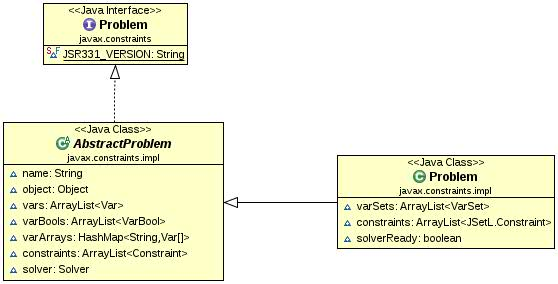
\includegraphics[scale=.5]{img/Problem.JPG}
\caption{Class Diagram di \texttt{Problem}.}
\end{figure}

\subsection{Implementazione}
Una volta definita la classe, come visto all'inizio 
della sezione \ref{problem}, sono stati inseriti tutti i metodi astratti
dell'interfaccia \files{Problem} non definiti nell'implementazione di base. 

Si descrivono ora gli attributi ed i metodi definiti, basati sul solver JSetL.

\subsubsection{Attributi}
Come accennato in precedenza, l'implementazione di base fornisce attributi
di classe per la gestione di variabili intere, booleane e per i vincoli, ma
non prevede nulla per quelle insiemistiche. Sono stati quindi aggiunti,
sulla base del medesimo meccanismo di \files{AbstractProblem}, attributi
per la gestione di queste variabili.
\begin{lstlisting}[language = Java,
                   caption = {attributi di \texttt{Problem}.}]
ArrayList<VarSet> varSets;

private static final int OPER_EQ = 1, OPER_UNKNOWN = 0, OPER_NEQ = 2, OPER_LT = 3, OPER_LEQ = 4, OPER_GT = 5, OPER_GEQ = 6;

private static int counter = 0;
\end{lstlisting}
L'attributo
\files{varSets} rappresenta la lista delle variabili insiemistiche appartenenti 
al problema. 

Sono state poi definite delle costanti utili per identificare gli operatori
($=$, $\leq$, $\geq$, $\ldots$) 
mediante il costrutto \files{switch} (che richiede come parametro un intero) e
delle variabili globali utilizzate per contare variabili interne al fine di 
assegnare un nome univoco alle stesse.

\subsubsection{Costruttori} 
I costruttori richiesti sono due: uno senza parametro ed uno con parametro
\files{String} che ne rappresenta il nome.
\begin{lstlisting}[language = Java,
                   caption = {costruttore con parametro.}]
public Problem(String name) {
	super(name);
	varSets = new ArrayList<VarSet>();
}
\end{lstlisting}

In entrambi i casi viene chiamato il costruttore della classe astratta di base
con la sola differenza che quello senza parametro assegna un valore di
default al nome:
\begin{lstlisting}[language = Java, frame = single]
	super("_P"+(counter++));
\end{lstlisting} 
e quindi viene inizializzata la lista delle variabili proprie della classe, 
ovvero quelle insiemistiche che si sono ridefinite nella nostra implementazione.

\subsubsection{Metodo \texttt{postElement}}
L'interfaccia \files{Problem} specifica anche metodi  per creare vincoli 
che hanno a che fare con elementi di array di interi o di variabili vincolate
intere. Se una variabile logica intera \files{indexVar} ha la funzione di
indice all'interno di un array \files{v}, il risultato di un'operazione
\files{v[indexvar]} è un'altra variabile vincolata. Poiché Java
non supporta l'overloading dell'operatore ``\files{[]}'' l'interfaccia
standard utilizza questo metodo.

Vi sono quattro possibili definizioni di questo metodo:
\begin{lstlisting}[language = Java, frame = single]
  public Constraint postElement(int[], Var, String, int);
  public Constraint postElement(int[], Var, String, Var);
  public Constraint postElement(Var[], Var, String, int);
  public Constraint postElement(Var[], Var, String, Var);
\end{lstlisting}

Vediamo nel dettaglio solo uno di questi metodi poiché in tutti e quattro i casi
si utilizza la classe di supporto \texttt{Element} che rappresenta il vincolo 
specificato mediante i parametri del costruttore e che sarà definito in 
\ref{Element}.

\begin{lstlisting}[language = Java,
                   caption = {\files{postElement}, array di interi.}]
public Constraint postElement(
                int[] array, 
                javax.constraints.Var indexVar, 
                String oper, 
                int value) {
        if (indexVar.getMin() > array.length - 1 || indexVar.getMax() < 0)
                throw new RuntimeException("elementAt: invalid index variable");
        Element result = new Element(array, indexVar, oper, value);
        post(result);
        return result;
}
\end{lstlisting}
Innanzitutto viene controllato che il dominio della variabile indice sia
compatibile con il range dell'array, altrimenti viene lanciata un'eccezione.
Viene quindi istanziata la variabile \texttt{result} di tipo \texttt{Element}
con i medesimi parametri del metodo invocato. Questa variabile rappresenta il
vincolo:
\begin{center}
\lstinline$array[indexVar] oper value$,
\end{center}
che viene infine aggiunto al problema mediante il metodo \texttt{post}.

\subsubsection{Metodo \texttt{post}}
Un vincolo non ha effetto fino a che non viene inserito nel problema. Per 
fare ciò si utilizza il metodo \files{post}, che ha le seguenti dichiarazioni:
\begin{lstlisting}[language = Java, frame = single]
public Constraint post(int[], Var[], String, int);
public Constraint post(int[], Var[], String, Var);
public Constraint post(Var[], String, int);
public Constraint post(Var[], String, Var);
public Constraint post(Var, String, int);
public Constraint post(Var, String, Var);
public Constraint post(Constraint);
\end{lstlisting}
Ogni metodo \files{post} ha il medesimo approccio: costruisce il vincolo 
basandosi sul metodo \files{linear} (si entrerà
nel dettaglio nei prossimi paragrafi), lo pubblica nel solver JSetL mediante
la chiamata della specifica \files{post(Constraint)} ed infine
lo aggiunge ai vincoli del problema con il metodo \files{add}.

\begin{lstlisting}[language = Java,
                   caption = {\files{post}.},
                   label = codicepost]
public Constraint post(
                int[] array, 
                javax.constraints.Var[] vars, 
                String oper, 
                int value) {
        Constraint result = linear(array, vars, oper, value);
        post(result);
        add(result);
        return result;
}

public Constraint post(
                Var var, 
                String oper, 
                int value) {
	Constraint result = linear(var, oper, value);
	post(result);
	add(result);
	return result;
}
\end{lstlisting}
Nel listato \ref{codicepost} si possono notare due metodi \files{post} 
standard, uno per le 
variabili singole (il secondo) ed uno per array di variabili. Entrambi 
utilizzano il metodo \files{linear} e restituiscono il nuovo vincolo
creato. 

\begin{lstlisting}[language = Java,
                   caption = {\files{post(Constraint)}.}]
public void post(javax.constraints.Constraint constraint) {
        add(constraint);
        addJSetLConstraints((JSetL.Constraint) constraint.getImpl());
}
\end{lstlisting}
Questo è invece il metodo su cui tutti gli altri si basano per aggiungere
il vincolo creato al \texttt{Problem}. Viene invocata la funzione \texttt{add}
della classe base per aggiungere il vincolo JSR-331. Quindi mediante il
metodo \texttt{addJSetLConstraints} si inserisce il vincolo specifico di
JSetL all'array di supporto.
\begin{flushleft}
Anche la classe \files{Constraint} ha un metodo \files{post}, per cui è 
possibile creare un vincolo e quindi renderlo attivo con la seguente sintassi:
\begin{lstlisting}[language = Java, frame = single]
Constraint c = p.linear(x, ``<='', y);
c.post();
\end{lstlisting}
\end{flushleft}

\subsubsection{Metodi \texttt{linear}}\label{metLinear}
I vincoli che hanno a che fare con il confronto di espressioni vincolate
utilizzano gli operatori di confronto standard:
\[
\begin{array}{c|c}
\textbf{Stringa} & \textbf{Semantica} \\
\hline \hline
< & \textrm{minore stretto,} \\
<= & \textrm{minore o uguale,} \\
= & \textrm{uguale,} \\
>= & \textrm{maggiore o uguale,} \\
> & \textrm{maggiore stretto,} \\
!= & \textrm{diverso.} \\
\end{array}
\]

I metodi che implementano il confronto sono chiamati \files{linear} e vengono
usati, come accennato in precedenza, nelle definizioni di \files{post}. \`E
anche possibile per l'utente utilizzare direttamente \files{linear}, non sono 
infatti
metodi privati, e sono utili perché non aggiungono direttamente un vincolo
e le variabili al problema.

Vi sono quattro differenti metodi \files{linear}:
\begin{lstlisting}[language = Java, frame = single]
public Constraint linear(int[], Var[], String, int);
public Constraint linear(int[], Var[], String, Var);
public Constraint linear(Var, String, int);
public Constraint linear(Var, String, Var);
\end{lstlisting}
i primi due hanno a che fare con vettori di variabili vincolate, mentre gli 
altri ne gestiscono una sola. In entrambi i casi si effettua il confronto
con un intero o un'altra variabile vincolata.

\begin{lstlisting}[language = Java,
                   caption = {\files{linear}, con array di variabili.}]
public Constraint linear(
                int[] array, 
                javax.constraints.Var[] vars, 
                String oper, int value) {
        if (array.length != vars.length || array.length == 0)
                throw new RuntimeException(
                        "Coefficent and variable length must be equal and not zero.");
        Var scalprod = (Var) scalProd(array, vars);
        return new Linear(scalprod, oper, value);
}
\end{lstlisting}
Il metodo con i vettori, dopo aver verificato che le lunghezze siano 
compatibili e non nulle, genera il prodotto scalare tra i due array tale che
se $v_0, v_1, \ldots, v_{n-1}$ sono le variabili contenute in \files{vars} e
$a_0, a_1, \ldots, a_{n-1}$ sono i coefficienti interi contenuti in 
\files{array},
la variabile vincolata $s$ rappresentata da \files{scalprod} è data da:
\[
s = a_0\cdot v_0 + a_1\cdot v_1 + \cdots + a_{n-1}\cdot v_{n-1}.
\]

Una volta creata la variabile temporanea \files{scalprod} viene calcolato 
e ritornato il vincolo mediante il costruttore della classe \texttt{Linear}.

\begin{lstlisting}[language = Java,
                   caption = {\files{linear}, con variabile singola.}]
public Constraint linear(
                javax.constraints.Var var, 
                String oper, 
                int value) {
        if (var == null)
                throw new RuntimeException("Parameters must not be null.");
        return new Linear(var, oper, value);
}
\end{lstlisting}
Nel metodo con la singola variabile viene controllato che \files{var} non sia
nulla, nel qual caso viene lanciata un'eccezione, anche quindi viene ritornata
la costruzione di un nuovo vincolo specifico di tipo \texttt{Linear}, discusso
nella sezione \ref{Linear}.

\subsubsection{Metodo \texttt{scalProd}}
Questo metodo pubblico permette di creare una nuova variabile vincolata
intera che rappresenta il prodotto scalare tra gli elementi degli array
passati come parametro. Come si è già visto per il metodo \files{linear} il
risultato che si ottiene è del tipo:
\[
s = a_0\cdot v_0 + a_1\cdot v_1 + \cdots + a_{n-1}\cdot v_{n-1}.
\]

\files{scalProd} è spesso utilizzato all'interno di altri metodi, ma è comunque
definito pubblicamente poiché rappresenta un'operazione comune per le variabili.

\begin{lstlisting}[language = Java,
                   caption = {\files{scalProd}.}]
public Var scalProd(int[] values, Var[] vars) {
  .
  .
  IntLVar[] intVars = new IntLVar[vars.length];
  if (values[0] != 0)
    intVars[0] = ((Var) vars[0]).getIntLVar().mul(values[0]);
  else intVars[0] = new IntLVar(0,0);
  for (int i = 1; i < values.length; i++) {
    if (values[i] !=0) {
      IntLVar tmp = new IntLVar(((Var) vars[i]).getIntLVar().mul(values[i]));
      intVars[i] = intVars[i-1].sum(tmp);
    }
    else intVars[i] = intVars[i-1];
  }
  return new Var(this, intVars[vars.length-1]);
}
\end{lstlisting}
Inizialmente il metodo controlla le lunghezze degli array (parte omessa) e se
non compatibili o se nulli lancia una \texttt{Runtime Exception}.

Quindi viene creato un array ausiliario di \files{IntLVar} di lunghezza pari
a quella dei due vettori \files{vars} e \files{values}. Questo vettore viene
utilizzato per calcolare i risultati parziali, ovvero nell'$i$-esimo elemento
è contenuto il prodotto scalare dei primi $i+1$ elementi.
\[
\begin{array}{rcl}
\files{vars} & = & [v_0, v_1, \ldots, v_i, \ldots, v_{n-1}] \\
\files{values} & = &  [a_0, a_1, \ldots, a_i, \ldots, a_{n-1}] \\
\hline
\hline
\files{intVars[i]} & = & a_0\cdot v_0 + a_1\cdot v_1 + \cdots + a_i\cdot v_i
\end{array}
\] 

Alla fine del processo si ottiene un array il cui ultimo elemento rappresenta
proprio il prodotto scalare dei due vettori passati come parametro.
A questo punto viene creata e restituita una nuova variabile intera JSR-331
mediante un opportuno costruttore.

\subsubsection{Metodo \texttt{allDifferent}}
L'interfaccia \files{Problem} definisce un modo semplice per creare ed inserire
nel problema uno dei più comuni vincoli globali conosciuto come AllDifferent:
\begin{center}
\lstinline[language = Java]$public Constraint postAllDifferent(Var[] vars);$
\end{center}
\`E definito un altro sinonimo più compatto:
\begin{center}
\lstinline[language = Java]$public Constraint postAllDiff(Var[] vars);$
\end{center}
Questi metodi creano, inseriscono nel problema e restituiscono un nuovo vincolo
per cui ogni variabile dell'array \files{vars} debba avere un valore diverso 
dalle altre.
La definizione del metodo è la seguente:
\begin{lstlisting}[language = Java,
                   caption = {\files{allDifferent}.}]
public Constraint postAllDifferent(Var[] vars) {
	if (vars.length == 0)
		throw new RuntimeException("Variable array must not be empty.");
	Constraint result = new AllDifferent(vars);
	post(result);
	return result;
}
\end{lstlisting}
Questo metodo crea semplicemente un nuovo vincolo appoggiandosi al costruttore 
della classe \files{AllDifferent} che verrà definito nella sezione 
\ref{AllDifferent}.

\subsubsection{Metodi \texttt{postCardinality}}
La specifica JSR-331 include tra i metodi pubblici alcune funzioni che
creano vincoli inerenti alla cardinalità di array di variabili
intere. Questi vincoli detti di cardinalità (\texttt{Cardinality Constraints}), 
che tuttavia non hanno nulla a che fare con le variabili insiemistiche, sono
quattro:
\begin{lstlisting}[language = Java, frame = single]
public Constraint postCardinality(Var[], int, String, int);
public Constraint postCardinality(Var[], int, String, Var);
public Constraint postCardinality(Var[], Var, String, int);
public Constraint postCardinality(Var[], Var, String, Var);
\end{lstlisting}

Poiché sono vincoli abbastanza particolari, la loro trattazione più dettagliata
viene fatta a parte, nella sezione \ref{Cardinality} per quanto riguarda la
classe \texttt{Cardinality} e nell'appendice \ref{cardinality} per l'approccio
e la trattazione del problema d'implementazione di tale vincolo.

\subsubsection{Metodi \texttt{postGlobalCardinality}}
L'interfaccia \files{Problem} specifica anche metodi utili per creare vincoli
di cardinalità globale noti come \emph{GCC} (\emph{Global Cardinality 
Constraints}) che rappresentano non uno, ma più
vincoli di cardinalità allo stesso tempo. La specifica prevede che il livello
d'implementazione di questi possa essere comune o specifico, ovvero è 
fornita un'implementazione nella classe \files{AbstractProblem}. \`E quindi
possibile implementare o meno questi metodi. 

La lista dei metodi, limitata alle variabili intere è la seguente:
\begin{lstlisting}[language = Java, frame = single]
public Constraint postGlobalCardinality(Var[], int[], Var[]);
public Constraint postGlobalCardinality(Var[], int[], int[], int[]);
\end{lstlisting}

In entrambi i casi il metodo sfrutta la costruzione di un vincolo
specifico implementato mediante la classe \texttt{GlobalCardinality} che verrà
definito in \ref{GlobalCardinality}.

\begin{lstlisting}[language = Java,
                   caption = {\files{postGlobalcardinality}.}]
public Constraint postGlobalCardinality(
                Var[] vars, 
                int[] values, 
                Var[] cardinalityVars) {
        Constraint c = new GlobalCardinality(vars, values, cardinalityVars);
        c.post();
        return c;
}
\end{lstlisting}
In questo esempio si può notare che il costruttore utilizza esattamente i 
parametri d'invocazione della funzione. Il vincolo creato viene quindi inserito
nel problema.

\section{Interfaccia comune: \texttt{CommonBase}}\label{common}
Prima di parlare nello specifico delle componenti del problema (inteso come CSP)
e quindi di variabili e vincoli, occorre parlare dell'interfaccia comune.
Come per l'interfaccia \files{Problem} anche le interfacce \files{Var},
\files{VarBool}, \files{VarSet} e \files{Constraint} sono fornite di
un'implementazione astratta (non pura) che fornisce attributi, costrutti e 
metodi di base. Questa è la classe \files{CommonBase}.

\subsection{Attributi}
Gli attributi della classe \files{CommonBase} sono quattro:
\begin{lstlisting}[language = Java, frame = single]
	Problem problem;
	String  name;
	Object  impl;
	Object  businessObject;
\end{lstlisting}
L'attributo
\files{problem} rappresenta il problema a cui l'oggetto del CSP è associato,
la stringa \files{name} è il nome dato all'oggetto. Si parla di oggetto
perché questa classe implementa gli attributi di base di ogni oggetto di un
CSP, ed è chiaro che ogni variabile intera, booleana o insiemistica possa avere
un nome, e \emph{debba} sicuramente avere un problema associato e una
parte implementativa.

La parte implementativa è rappresentata dall'attributo \files{impl}, che per
l'appunto è un'istanza \files{Object}, ovvero l'oggetto generico Java. Ogni
implementazione specifica (come JSetL) deve, se supportato, appoggiarsi
all'attributo \files{impl} per sfruttare la propria implementazione.

L'ultimo attributo della classe è \files{businessObject}, che può essere
utilizzato come attributo di supporto per le specifiche implementazioni.

\subsection{Costruttori}
Con la classe \files{CommonBase} vengono forniti due costruttori, uno senza 
parametro ed uno con parametro stringa che ne rappresenta il nome.
\begin{lstlisting}[language = Java,
                   caption = {costruttori di \files{CommonBase}.},
                   label = list01]
public CommonBase(Problem problem) {
	this(problem,"");
}

public CommonBase(Problem problem, String name) {
	this.problem = problem;
	this.name = name;
	impl = null;
	businessObject = null;
}
\end{lstlisting}
Il primo costruttore definito nel listato \ref{list01} si limita a chiamare il 
secondo passando come parametro la stringa vuota. Quest'ultimo imposta il
problema ed il nome passati come parametro ai relativi attributi \files{problem}
e \files{name}, infine \files{impl} e \files{businessObject} vengono impostati
a \files{null}.

L'importanza di questi costruttori è dovuta al fatto che ogni classe derivata
dalla suddetta dovrà utilizzarli. Questo implica che ogni classe
(\files{Var}, \files{VarBool}, \files{VarSet} e
\files{Constraint}) dovrà fornire tali costruttori di base ed 
utilizzare quindi il metodo \files{setImpl} per definire la propria
implementazione dell'oggetto costruito.  


\subsection{Metodi}
La classe \files{CommonBase} fornisce alcuni metodi comuni per qualsiasi tipo
di variabile o vincolo. Se ne descrivono brevemente alcuni.
\begin{itemize}
\item[-]\lstinline[language = Java]$public Problem getProblem()$

Restituisce il problema a cui l'oggetto
d'invocazione è legato.

\item[-]\lstinline[language = Java]$public void setName(String name)$

Imposta il nome dell'oggetto.

\item[-]\lstinline[language = Java]$public String getName()$

Restituisce il nome dell'oggetto
d'invocazione.

\item[-]\lstinline[language = Java]$public void setImpl(Object impl)$

Imposta l'implementazione concreta di uno 
specifico solver per l'oggetto d'invocazione.

\item[-]\lstinline[language = Java]$public Object getImpl()$

Restituisce l'implementazione concreta (dello 
specifico solver) per l'oggetto d'invocazione.

\item[-]\lstinline[language = Java]$public void setObject(Object obj)$

Aggiunge un oggetto ausiliari.

\item[-]\lstinline[language = Java]$public Object getObject()$ 

Restituisce l'oggetto ausiliario.
\end{itemize}


\section{Classe \texttt{Var}}
Questa classe implementa le variabili intere vincolate
\files{Var} per la specifica JSR-331
estendendo la classe \files{AbstractVar} (e quindi 
\files{CommonBase}).

Come visto nella descrizione dell'interfaccia comune vengono forniti tutti gli
attributi e metodi utili ed è quindi sufficiente implementare i metodi
dell'interfaccia \files{AbstractVar} ed i costruttori di \files{CommonBase},
mappando quindi le funzionalità richieste per la classe \files{Var}
con quelle fornite da JSetL (tramite \files{IntLVar}).

\begin{lstlisting}[language = Java,
                   frame = single,
                   caption = {metodi di Var},
                   label = metodiVar]
        public int getMin();
	public int getMax(); 
	public boolean isBound();
	public boolean contains(int value);
	public Var plus(int value);
	public Var minus(int value);
	public Var plus(Var x);
	public Var minus(Var x); 
	public Var multiply(int value);
	public Var multiply(Var x);
	public Var divide(int value);
	public Var divide(Var x);
\end{lstlisting}

\subsection{Costruttori}
Sono stati implementati vari costruttori per la classe \files{Var} atti
a soddisfare diverse esigenze, in primis quelle richieste dalla specifica e 
quindi altre suggerite dallo sviluppo del progetto.

Il meccanismo è simile per tutti i costruttori: si richiama il costruttore
della classe base (mediante il costrutto \files{super}) con il
parametro \files{Problem} (e a volte il nome), quindi si imposta l'oggetto
\files{impl} con l'implementazione concreta.
 
\begin{lstlisting}[language = Java,
                   caption = {un costruttore di \files{Var}.}]
public Var(Problem problem) {
	super(problem);
	String name = problem.getFreshName();
	setImpl(new IntLVar(name));
	setName(name);
}
\end{lstlisting}
In questo esempio si vede il costruttore con il solo parametro \files{problem}.
Viene chiamato il costruttore \files{AbstractVar(problem)} mediante il
costrutto \files{super(problem)}, quindi viene generato un nuovo nome mediante
la funzione di 
supporto \files{getFreshName}\footnote{\samepage La funzione ausiliaria 
\files{getFreshName} si limita a
creare un nome per le variabili interne che sia unico, al fine di rendere più
chiara la fase di debugging, non è trattata nel dettaglio.} della 
classe \files{Problem}.

A questo punto viene impostato l'attributo \files{impl} con una nuova istanza
della classe \files{IntLVar} creata con il costruttore con parametro stringa,
che ne rappresenta il nome, infine questo
viene settato anche per la variabile \files{Var}.

\begin{figure}[!ht]\label{varUML}
\centering
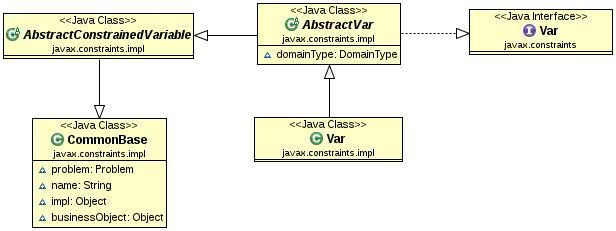
\includegraphics[scale=.5]{img/Var.JPG}
\caption{Class Diagram di \texttt{Var}.}
\end{figure}

\subsection{Metodi di uso generale}
I primi quattro metodi dell'elenco \ref{metodiVar} sono metodi di utilità 
generica e se ne dà una descrizione dettagliata.
\subsubsection{Metodo \texttt{getMin}}
Il metodo \files{getMin} restituisce il più piccolo intero del dominio
della variabile d'invocazione. \`E definito nel seguente modo:
\begin{lstlisting}[language = Java,
                   caption = {\files{getMin}.}]
public int getMin() {
	MultiInterval domain = ((IntLVar) getImpl()).getDomain();
	return domain.getGlb();
}
\end{lstlisting}
Dapprima viene presa l'implementazione concreta con il metodo \files{getImpl},
che in questo caso restituisce l'istanza di \files{IntLVar} relativa alla
variabile d'invocazione (\files{this}). A questo punto, mediante il metodo 
\files{getDomain},
dalla variabile si ottiene il dominio sotto forma di \files{MultiInterval}.
Viene quindi restituito il minimo valore di \files{domain} con il
metodo \files{MultiInterval.getGlb}.

\subsubsection{Metodo \texttt{getMax}}
Il metodo \files{getMax} restituisce il più grande intero del dominio
della variabile d'invocazione. \`E definito nel seguente modo:
\begin{lstlisting}[language = Java,
                   caption = {\files{getMax}.}]
public int getMin() {
	MultiInterval domain = ((IntLVar) getImpl()).getDomain();
	return domain.getGlb();
}
\end{lstlisting}
Analogamente a \files{getMin} questo metodo sfutta le funzionalità di
\files{IntLVar} e \files{MultiInterval}.

\subsubsection{Metodo \texttt{isBound}}
Il metodo \files{isBound}, come suggerisce il nome, è di tipo booleano, ovvero
ha due possibili valori di ritorno: \files{true} se il dominio della variabile
vincolata si riduce ad un singoletto, \files{false} altrimenti.
\begin{lstlisting}[language = Java,
                   caption = {\files{isBound}.}]
public boolean isBound() {
	return ((LVar) getImpl()).isBound();
}
\end{lstlisting}
Questo metodo si appoggia semplicemente al relativo metodo di JSetL per le
variabili intere.

\subsubsection{Metodo \texttt{contains}}
Anche questo è un metodo booleano, restituisce \files{true} se e solo se
un dato intero appartiene al dominio della variabile.
\begin{lstlisting}[language = Java,
                   caption = {\files{contains}.}]
public boolean contains(int value) {
	MultiInterval domain = ((IntLVar) getImpl()).getDomain();
	return domain.contains(value);
}
\end{lstlisting}
Come nei metodi precedenti viene prima richiamato il dominio della variabile
JSetL e in seguito viene ritornato il medesimo metodo sui multi-intervalli
\files{MultiInterval.contains(int)}.

\subsection{Operazioni aritmetiche}
La classe \files{AbstractVar} prevede l'implementazione dei comuni operatori
aritmetici per le variabili intere: ``$+$'', ``$\cdot$'', ``$-$'', ``$\div$''.

Per ogni operatore è definita una funzione con parametro intero ed una che abbia
come parametro un'altra variabile intera, questo permette di ottenere delle
espressioni del tipo:
\[
X + k, \quad X + Y,
\]
dove $X$ e $Y$ rappresentano delle variabili intere vincolate e $k$ un intero.

La lista dei metodi aritmetici è definita dalle ultime otto dichiarazioni
del listato \ref{metodiVar}, poiché si basano tutte sullo stesso principio ne
verranno definite nel dettaglio solo due, una con parametro intero ed
una con parametro variabile.

\begin{lstlisting}[language = Java,
                   caption = {\files{plus}, con parametro intero.}]
public Var plus(int value) {
	Problem p = (Problem) getProblem();
	Var x = new Var(p, p.getFreshName());
	x.setImpl(((IntLVar) getImpl()).sum(value));
	((IntLVar)x.getImpl()).setName(x.getName());
	// To constraint the new variable.
	Constraint c = new Constraint(p,
		((IntLVar) x.getImpl()).eq(((IntLVar) getImpl()).sum(value)));
	p.post(c);
        return x;
}
\end{lstlisting}
Il metodo crea una nuova variabile \files{x} di tipo \files{Var} che
poi verrà restituita come risultato, a questa viene assegnato un nuovo nome
e una nuova implementazione, vincolata ad essere il risultato della somma
della variabile d'invocazione e dell'intero \files{value}.

A questo punto si potrebbe dire che il lavoro sia finito e si possa
restituire il 
risultato, tuttavia si commetterebbe un errore. La nuova variabile deve infatti
essere vincolata ed è quindi necessario aggiungere al
solver JSetL il vincolo $X = T+k$ dove $X$ è la variabile creata, $T$ è
quella di invocazione e $k$ l'intero \files{value}.

Questa aggiunta (che, nel codice, è definita subito dopo il commento) è stata
dovuta non tanto per la correttezza del metodo per quanto riguarda le variabili
del problema, ma per le variabili di supporto i cui vincoli non verrebbero 
aggiornati all'interno del solver JSetL.

\begin{lstlisting}[language = Java,
                   caption = {\files{multiply}, con parametro variabile.}]
public Var multiply(javax.constraints.Var x) {
        Problem p = (Problem) getProblem();
        Var a = new Var(p, p.getFreshName());
        a.setImpl(((IntLVar) getImpl()).mul(((Var) x).getIntLVar()));
        ((IntLVar)a.getImpl()).setName(a.getName());
        // To constraint the new variable.
        Constraint c = new Constraint(p,
             ((IntLVar) a.getImpl()).eq(((IntLVar) getImpl()).mul((IntLVar) x.getImpl())));
        p.post(c);
        return a;
}
\end{lstlisting}
Come si può notare il metodo con parametro variabile è sostanzialmente identico,
l'unica differenza è data dalla chiamata della funzione \files{getImpl}
per il parametro \files{x} all'interno del costruttore del nuovo vincolo
inserito.

\section{Classe \texttt{VarBool}}
La classe \files{VarBool} rappresenta le variabili booleane. Queste si 
possono considerare un caso particolare 
delle variabili intere, con il dominio ristretto ai valori $[0,1]$. In cui
$0$ rappresenta il valore \files{false} e $1$ il valore \files{true}.

JSR-331 fornisce un'implementazione di base per questa classe che estende
\files{Var}, tuttavia si è scelto di ridefinirla (anche se in modo del tutto
analogo) per avere una gestione più diretta e per facilitare eventuali
modifiche future.
\begin{lstlisting}[language = Java, frame = single]
public class VarBool extends Var implements VarBool {
\end{lstlisting}
\subsection{Costruttori}
I costruttori della classe chiamano quelli della classe base
\files{Var} e quindi impostano l'implementazione con una variabile dal
dominio $[0,1]$
\begin{lstlisting}[language = Java,
                   caption = {un costruttore di \files{VarBool}}]
public VarBool(Problem problem, String name) {
	super(problem, name);
	setImpl(new IntLVar(name, 0, 1));
}
\end{lstlisting}

\section{Classe \texttt{VarSet}}
La specifica JSR-331 introduce un'interfaccia basilare per le variabili
insiemistiche vincolate. Al contrario delle variabili intere, quando un'istanza
 di questa classe è considerata bound  significa che coincide ad un 
singolo insieme di
valori interi.

Il pacchetto \files{javax.constraints.impl} fornisce la classe 
\files{BasicVarSet} che di fatto implementa l'interfaccia \files{VarSet}. 
Tuttavia poiché JSetL ha le proprie classi che implementano insiemi, 
e soprattutto insiemi di interi mediante la classe \files{SetLVar}, si è deciso
di non considerare l'implementazione di base fornita e proseguire con 
l'approccio utilizzato per la classe \files{Var}.
\begin{lstlisting}[language = Java,
                   frame = single]
public class VarSet extends AbstractConstrainedVariable 
    implements javax.constraints.VarSet {
\end{lstlisting}

La classe estende \files{AbstractConstrainedVariable} e quindi 
\texttt{CommonBase}  che come si è già più volte
sottolineato, fornisce tutti gli strumenti necessari. Inoltre 
\files{VarSet} implementa direttamente l'interfaccia \files{VarSet}, al
contrario di quanto visto per la classe \texttt{Var}.


\begin{figure}[!ht]\label{varsetUML}
\centering
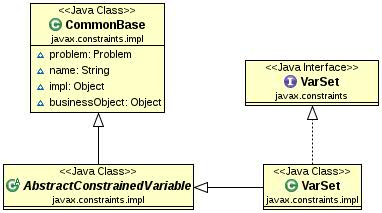
\includegraphics[scale=.75]{img/VarSet.JPG}
\caption{Class Diagram di \texttt{VarSet}.}
\end{figure}

\begin{flushleft}
Il dominio di una variabile insiemistica consiste in due insiemi:
\begin{enumerate}
\item[-]Required Set: un insieme di interi i cui valori appartengono
 tutti alla variabile (lower bound);
\item[-]Possibile Set: un insieme di interi in cui almeno un valore
appartiene alla variabile (upper bound).
\end{enumerate}
\end{flushleft}
Il Required Set è sempre un sottoinsieme del Possibile Set. Ad esempio,
se una variabile insiemistica rappresenta i giorni lavorativi della settimana, 
i valori possibili sono: $\{1, 2, 3, 4, 5, 6, 7 \}$, mentre quelli richiesti
dovranno essere un sottoinsieme di cardinalità $5$, ad esempio 
$\{1, 2, 3, 4, 5\}$. 
\`E permesso rimuovere elementi solo dai valori possibili ed
aggiungerli solo a quelli richiesti. La cardinalità di una variabile
insiemistica vincolata è una variabile intera vincolata. \`E possibile definire
intersezione ed unione di variabili insiemistiche.


Se chiamiamo $V$ una generica variabile insiemistica, $L$ e $U$ due insiemi di
interi che rappresentano rispettivamente Required Set e Possibile Set,
tale che $L \subseteq U$, allora il dominio di $V$ si può esprimere nel
seguente modo:
\[
\textrm{dom}(V) = \{L,U\}.
\]
\begin{flushleft}
Tutte queste caratteristiche, specificate nel documento di riferimento di
JSR-331 \cite{specifiche}, sono già presenti nella classe \files{SetLVar} di 
JSetL, ed è
stato quindi semplice e naturale sfruttarne le caratteristiche.
\end{flushleft}
\subsection{Costruttori}
I costruttori richiesti dall'interfaccia sono solo quelli definiti in
\files{CommonBase}, infatti \files{VarSet} non ne prevede dei propri. I 
costruttori standard sono:
\begin{lstlisting}[language = Java,
                   frame = single]
public VarSet(Problem);
public VarSet(Problem, String);
\end{lstlisting}
mentre quelli definiti in un secondo momento, per venire incontro alle 
necessità implementative sono:
\begin{lstlisting}[language = Java,
                   frame = single]
public VarSet(Problem,  int[], String);
public VarSet(Problem, Set<Integer>, Set<Integer>, String);
public VarSet(Problem, MultiInterval, String);
public VarSet(Problem, SetLVar);
\end{lstlisting}

Come per la classe \files{Var} ogni costruttore utilizza il medesimo
approccio: viene chiamato il costruttore della classe base  mediante il 
costrutto
\files{super} e quindi viene impostato l'oggetto \files{impl} con
una chiama al relativo costruttore di \files{SetLVar}.

Si danno alcuni esempi.

\begin{lstlisting}[language = Java,
                   caption = {un costruttore standard di \files{VarSet}}]
public VarSet(Problem problem, String name) {
	super(problem);
	setImpl(new SetLVar(name));
	setName(name);
}
\end{lstlisting}
Il costruttore in questione si comporta esattamente come quello definito per
la classe \files{Var}.

\begin{lstlisting}[language = Java,
                   caption = {costruttore con lista di interi.}]
public VarSet(Problem problem,  int[] values, String name) {
	super(problem, name);
	MultiInterval s = new MultiInterval();
	for (int i = 0; i < values.length; i++)
		s.add(values[i]);
	setImpl(new SetLVar(name,s));
}
\end{lstlisting}
In questo costruttore, che ha come parametro una lista di interi ed il nome,
viene creato un multi-intervallo a cui vengono aggiunti uno ad uno tutti gli
elementi dell'array \files{values}. Quindi viene chiamato il costruttore
che ha come parametro un \files{MultiInterval} fornito da JSetL.


\begin{lstlisting}[language = Java,
                   caption = {costruttore con un multi-intervallo.}]
public VarSet(Problem problem, MultiInterval lb, String name) {
	super(problem, name);
	setImpl(new SetLVar(name, lb, MultiInterval.universe()));
}
\end{lstlisting}
Questo costruttore ausiliario sfrutta la classe JSetL \files{MultiInterval}
di cui si è già spesso parlato e che è definita in \cite{tesiAmadini}. 
In questo caso
viene chiamato un costruttore di \files{SetLVar} che utilizza due 
multi-intervalli, il primo rappresenta i valori opzionali, mentre
il secondo quelli richiesti.

Sia $L$ l'insieme che rappresenta il multi-intervallo \files{lb}, $\mathcal{U}$
l'insieme universo (di tutti gli interi rapprensentabili dall'implementazione),
allora la variabile insiemistica creata $V$ ha dominio:
\[
\textrm{dom}(V) = \{ L, \mathcal{U} \}.
\] 

\subsection{Metodi di uso generale}
L'interfaccia \files{VarSet} prevede alcuni metodi di utilità generica, tra cui
si evidenziano:
\begin{lstlisting}[language = Java,frame = single]
public boolean isBound();
public Set<Integer> getValue() throws Exception;
public void setValue(Set<Integer> set) throws Exception;
public Set<Integer> getRequiredSet();
public Set<Integer> getPossibleSet();
public boolean isPossible(int value);
public boolean isRequired(int value);
public void remove(int value) throws Exception;
public void require(int val) throws Exception;
public boolean contains(Set<Integer> setOfValues);
public void setEmpty(boolean flag);
public Var getCardinality();
\end{lstlisting}
Alcuni di questi metodi si avvalgono della controparte nell'implementazione
concreta  JSetL e quindi non se ne darà la definizione. Tra questi
si ha \files{isBound}, \files{getValue} e \files{setValue}.

I metodi che hanno a che fare con il dominio invece seguono un altro approccio,
dovendosi basare sulla funzione \files{getDomain} che restituisce il
dominio della variabile JSetL \files{SetLVar}. Questo dominio è
un'istanza della classe \files{SetInterval} e quindi i metodi sono basati su
questa classe oltre che sui multi-intervalli già citati.

\begin{lstlisting}[language = Java,
                   caption = {metodi getter per il dominio.}]
public Set<Integer> getRequiredSet() {
	return ((SetLVar) getImpl()).getDomain().getGlb();
}

public Set<Integer> getPossibleSet() {
	return ((SetLVar) getImpl()).getDomain().getLub();
}
\end{lstlisting}
Come anticipato la chiave dei metodi \files{getRequiredSet} e 
\files{getPossibleSet} è una funzione della classe
\files{SetInterval} che rappresenta il dominio di una variabile insiemistica.
Con \files{getGlb} viene restituito un multi-intervallo (che implementa un
\files{Set<Integer>}) rappresentante il lower-bound della variabile.
Invece \files{getLub} restituisce l'upper-bound. I due oggetti
mappano perfettamente l'insieme required e possible definiti in \files{VarSet}.

\begin{lstlisting}[language = Java,
                   caption = {un intero è possibile o richiesto?.}]
public boolean isPossible(int value) {
	return ((SetLVar) getImpl()).getDomain().getLub().contains(value);
}

public boolean isRequired(int value) {
	return ((SetLVar) getImpl()).getDomain().getGlb().contains(value);
}
\end{lstlisting}
Nelle funzioni \files{isPossible} e \files{isRequired}, dopo aver ottenuto 
l'insieme required o possible viene utilizzato
 il metodo \files{contains} che restituisce un booleano a seconda che
l'intero passato come parametro sia contenuto nel multi-intervallo di 
invocazione o meno.

\begin{lstlisting}[language = Java,
                   caption = {inserire e rimuovere elementi.}]
public void remove(int value) throws Exception {
	((SetLVar) getImpl()).getDomain().getLub().remove(value);	
}

public void require(int value) throws Exception {
	((SetLVar) getImpl()).getDomain().getGlb().add(value);	
}
\end{lstlisting}
Nella descrizione inziale della classe si è detto che è 
permesso rimuovere elementi solo dai valori possibili ed aggiungerli solo a
quelli richiesti. I metodi \files{remove} e \files{require} implementano 
quanto detto, non sono
state quindi fornite funzioni che aggiungano elementi all'upper-bound
o ne rimuovano dal lower-bound.

\begin{lstlisting}[language = Java,
                   caption = {inclusione insiemistica.}]
public boolean contains(Set<Integer> setOfValues) {
	return ((SetLVar) getImpl()).getDomain().getLub().containsAll(setOfValues);
}
\end{lstlisting}
Il metodo booleano \files{contains} controlla se ogni elemento dell'insieme
dato sia contenuto nel dominio della variabile d'invocazione. 
Utilizza il metodo \files{containsAll} sui multi-intervalli.

\begin{lstlisting}[language = Java,
                   caption = {getter per la cardinalità.}]
public Var getCardinality() {
	Var result = new Var((Problem) getProblem(), ((SetLVar) getImpl()).card());
	return result;
}
\end{lstlisting}
Il metodo \files{getCardinality} si avvale del metodo \files{card} presente 
nella  classe \files{SetLVar}, che
restituisce una variabile vincolata intera rappresentante la cardinalità 
dell'insieme. Questa variabile viene poi utilizzata per costruire una nuova
variabile intera \files{Var}  che viene quindi
restituita dal metodo.

\subsection{Operazioni insiemistiche}
\files{VarSet} prevede le operazioni insiemistiche di unione ed intersezione.
Queste operazioni sono già presenti in \files{SetLVar} ed è stato quindi 
semplice implementarle. JSetL prevede inoltre le operazioni di complementazione
e differenza insiemistica al contrario dello standard, tuttavia non è stata
fornita una implementazione per queste.

\begin{lstlisting}[language = Java,
                   caption = {unione insiemistica.}]
public VarSet union(javax.constraints.VarSet varSet) {
        Problem p = (Problem) getProblem();
        SetLVar tmp = ((SetLVar) varSet.getImpl());
        VarSet result = new VarSet(p);
        result.setImpl(((SetLVar)getImpl()).union(tmp));
        // To constraint the new variable.
        Constraint c = new Constraint(p,
                ((SetLVar) result.getImpl()).eq(((SetLVar)getImpl()).union(tmp)));
        p.post(c);
        return result;
}
\end{lstlisting}

\begin{lstlisting}[language = Java,
                   caption = {intersezione insiemistica.}]
public VarSet intersection(javax.constraints.VarSet varSet) {
        Problem p = (Problem) getProblem();
        SetLVar tmp = ((SetLVar) varSet.getImpl());
        VarSet result = new VarSet(p);
        result.setImpl(((SetLVar)this.getImpl()).intersect(tmp));
        // To constraint the new variable.
        Constraint c = new Constraint(p, ((SetLVar) result.getImpl()).eq(
                        ((SetLVar)getImpl()).intersect(tmp)));
        p.post(c);
        return result;
}
\end{lstlisting}
In entrambi i metodi si dichiara una variabile temporanea di tipo 
\files{SetLVar} che rappresenti la variabile passata come parametro e quindi si 
crea la variabile di tipo \files{VarSet} che diventerà il risultato 
dell'operazione. A \files{result} viene assegnato il risultato
dell'operazione tra la variabile temporanea e la variabile d'invocazione 
concreta. Anche in questo caso, come per le operazioni aritmetiche sulle
variabili intere, occorre aggiornare i vincoli per la nuova variabile creata.
Il sistema utilizzato è quindi il medesimo.


\section{Classe \texttt{Constraint}}\label{constraint}
L'ultima classe che si tratta a riguardo della definizione del problema è
quella che rappresenta il vincolo generico. JSR-331 specifica i vincoli più
comuni che definiscono relazioni tra variabili. Questi vincoli
possono essere ottenuti tramite l'interfaccia \files{Problem} ed ognuno di
essi è un' istanza di questa classe.

\subsection{Implementazione}
\files{Constraint} implementa i vincoli JSR-331 estendendo la classe
astratta dell'implementazione.
\begin{lstlisting}[language = Java,frame = single]
abstract public class AbstractConstraint extends CommonBase implements javax.constraints.Constraint {
\end{lstlisting}
Come si può vedere \files{AbstractConstraint} a sua volta estende 
\files{CommonBase}, già descritta nella sezione \ref{common}. Questo vuol dire 
che ogni attributo e metodo utile è ereditato dalla classe e verrà quindi 
sfruttato nell'implementazione. Si hanno poi i metodi definiti nella classe 
astratta: \files{post},  \files{and},  \files{or},  \files{negation} e
 \files{implies}; a parte il primo sono tutti stati ridefiniti poiché JSetL
fornisce la propria implementazione.

\subsection{Costruttori}
Analogamente a quanto visto per gli altri elementi del problema (le variabili)
i costruttori di questa classe richiedono come parametro il problema.
Viene poi fornito un costruttore che aggiunge il nome ed infine uno ausiliario
per l'implementazione JSetL.

\begin{lstlisting}[language = Java,
                   caption = {i costruttori.}]
public Constraint(Problem problem) {
	super(problem);
	setImpl(new JSetL.Constraint());
}

public Constraint(Problem problem, String name) {
	super(problem, name);
	setImpl(new JSetL.Constraint());
}

public Constraint(Problem problem, JSetL.Constraint constraint) {
	super(problem);
	setImpl(constraint);
}
\end{lstlisting}
I tre costruttori sopra definiti utilizzano il medesimo approccio di ogni
classe che si basa su \files{CommonBase}: chiamano il costruttore base e
quindi impostano l'implementazione concreta di JSetL.

\subsection{Vincoli logici}
La specifica JSR-331 prevede quattro metodi che rappresentano i comuni
operatori logici per creare vincoli: $\wedge$, $\vee$, $\neg$ e $\Rightarrow$.

Siano $\mathcal{C}_1$ e $\mathcal{C}_2$ generici vincoli, allora le seguenti
espressioni sono a loro volta vincoli:
\begin{center}
$\mathcal{C}_1 \wedge \mathcal{C}_2$,\quad
$\mathcal{C}_1 \vee \mathcal{C}_2$, \quad
$\neg \mathcal{C}_1$, \quad
$\mathcal{C}_1 \Rightarrow \mathcal{C}_2$.
\end{center}

\subsubsection{Congiunzione logica}
La congiunzione logica è implementata tramite il metodo \files{and} ed ha un
parametro di tipo \files{Constraint}:
\begin{lstlisting}[language = Java,
                   caption = {\files{and}.}]
public Constraint and(Constraint c) {
	JSetL.Constraint constraint = ((Constraint) c).getConstraint();
	Constraint result = new Constraint(getProblem(), this.getConstraint().and(constraint));
	return result;
}
\end{lstlisting}
Il metodo semplicemente crea un nuovo vincolo mediante il costruttore ausiliario
creato per JSetL. Utilizza il metodo \files{and} della classe
\files{Constraint} di JSetL.

\subsubsection{Disgiunzione logica}
Anche la disgiunzione logica ha un vincolo come parametro ed è implementata 
dal seguente codice: 
\begin{lstlisting}[language = Java,
                   caption = {\files{or}.}]
public Constraint or(Constraint c) {
	JSetL.Constraint constraint = ((Constraint) c).getConstraint();
	Constraint result = new Constraint(getProblem(), this.getConstraint().or(constraint));
	return result;		
}
\end{lstlisting}
Il metodo è praticamente identico al primo, con l'unica differenza che nel
costruttore è utilizzato il metodo \files{or}. 

\subsubsection{Negazione}
La Negazione, contrariamente agli altri metodi, non ha argomenti, per il 
resto è identico come approccio: viene creato un nuovo vincolo
mediante il metodo \files{notTest}:
\begin{lstlisting}[language = Java,
                   caption = {\files{negation}.}]
public Constraint negation() {
	Constraint result = new Constraint(getProblem(), this.getConstraint().notTest());
	return result;		
}
\end{lstlisting}

\subsubsection{Implicazione}
L'implicazione segue di pari passo i primi due metodi descritti: ha un parametro
di tipo \files{Constraint} e crea un nuovo vincolo mediante il metodo
\files{impliesTest} di JSetL.
\begin{lstlisting}[language = Java,
                   caption = {\files{implies}.}]
public Constraint implies(Constraint c) {	
	JSetL.Constraint constraint = ((Constraint) c).getConstraint();
	Constraint result = new Constraint(getProblem(), this.getConstraint().impliesTest(constraint));
	return result;
}
\end{lstlisting}
\begin{nota}
Nella classe \files{JSetL.Constraint} erano presenti i soli metodi \files{or} e
\files{and} che implementavano la disgiunzione e congiunzione logica
(la disgiunzione viene propagata in modo 
non deterministico). Durante lo sviluppo dell'interfaccia per la specifica si
è reso necessaria l'introduzione di metodi per
la negazione e l'implicazione.

Sono stati quindi forniti i metodi \files{impliesTest}, e
\files{notTest} che realizzano un'implementazione deterministica delle
relative operazioni logiche.

Nell'approccio di JSetL per la soluzione dei vincoli il non determinismo 
garantisce il risultato a scapito dell'efficienza; tuttavia sono stati 
introdotti altri sistemi per raggiungere la correttezza e la completezza, come 
il labeling visto nel capitolo \ref{jsetl}.

L'approccio nello sviluppo dell'implementazione JSR-331 basata su JSetL verte 
sul labeling di ogni
variabile inserita nel problema e questo garantisce un risultato quando si
cerca una soluzione. Per questo motivo l'utilizzo di metodi  deterministici
non è un problema, anzi in alcuni test si è rivelato un approccio molto
più efficiente.
\end{nota}

\section{Vincoli specifici}\label{nuoviConstraint}
Durante il testing mediante TCK e con l'esecuzione di alcuni
esempi inclusi nella cartella \files{sample} dello stesso si è resa necessaria
l'implementazione di alcune classi non incluse nel documento di specifica:
\begin{itemize}
  \item[-]\files{AllDifferent.java}
  \item[-]\files{And.java}
  \item[-]\files{Cardinality.java}
  \item[-]\files{Element.java}
  \item[-]\files{GlobalCardinality.java}
  \item[-]\files{IfThen.java}
  \item[-]\files{Linear.java}
  \item[-]\files{Neg.java}
  \item[-]\files{Or.java}
\end{itemize}

Ogniuna di queste estende la classe \files{Constraint} e ne ridefinisce i 
costruttori in modo
tale che rappresenti un ben definito vincolo. Alcune di queste classi sono 
utilizzate
nelle definizioni dei vari metodi della classe \texttt{Problem} per la
creazione e l'inserimento di vincoli relativi al problema, altre invece ne
sfruttano le peculiarità.

Poiché ogni classe che implementa vincoli specifici estende 
\texttt{Constraints} non saranno date tutte le definizioni di classe, se ne
fornisce una a fine esemplificativo:
\begin{lstlisting}[language = Java,frame = single]
public class Linear extends Constraint {
\end{lstlisting}
Verranno quindi di seguito, per ogni vincolo, descritti i costruttori più
significativi.

\subsection{Classe \texttt{Linear}}\label{Linear}
Questa classe rappresenta il più classico vincolo sulle variabili logiche
intere, ovvero il vincolo lineare. JSR-331 prevede quattro possibili
vincoli come descritto nella sezione \ref{metLinear}. 

I costruttori che hanno come parametri array di interi e variabili funzionano
esattamente come il metodo \texttt{scalProd} definito all'interno della
classe \texttt{Problem}. L'unica differenza è che una volta computata la
variabile rappresentante il prodotto scalare questa viene vincolata al valore
o alla variabile passata come parametro mediante l'operatore dato, esattamente
come verrà descritto di seguito.
Non se ne darà quindi una descrizione dettagliata.

Per quanto riguarda i costruttori con variabili singole si dà la definizione
di uno solo dei metodi poiché pressoché identici. Entrambi hanno come primo
parametro una variabile \texttt{var} o \texttt{var1}, come secondo una stringa 
\texttt{oper} e come terzo ed ultimo una variabile \texttt{var2} o un intero
\texttt{value}.
La stringa \files{oper} rappresenta
l'operatore di confronto che viene gestito dalla funzione \files{getOperator},
su cui non ci si soffermerà.

\begin{lstlisting}[language = Java,
                   caption = {costruttore \files{Linear} 
                   con variabile e intero.}]
public Linear(javax.constraints.Var var, String oper, int value) {
        super(var.getProblem());
	IntLVar v = ((Var) var).getIntLVar();
	switch(getOperator(oper)) {
	case 1: {
		// Case = "equals".
		JSetL.Constraint constraint = v.eq(value);
		setImpl(constraint);
	} break;
	case 2: {
		// Case != "not equals".
		JSetL.Constraint constraint = v.neq(value);
		setImpl(constraint);
	} break;
        .
        .
        .
	case 6: {
		// Case >= "greater equals".
		JSetL.Constraint constraint = v.ge(value);
		setImpl(constraint);
	} break;
	default: throw new UnsupportedOperationException();
	}
}
\end{lstlisting}
Inizialmente viene chiamato il costruttore della classe base con l'istanza
della classe \texttt{Problem} della variabile passata come parametro.
Quindi viene estratta la variabile intera JSetL di tipo 
\files{IntLVar} mediante la funzione ausiliaria \files{getIntLVar} (che non
fa altro che chiamare il metodo \files{getImpl} dell'implementazione comune).
Quindi, a seconda del caso, viene creato un vincolo JSetL opportuno 
(nel listato, per leggibilità,
sono stati omessi alcuni casi) utilizzato per essere impostato come
implementazione del vincolo creato mediante il metodo \texttt{setImpl}.
\begin{flushleft}
Ecco un'istruzione JSetL per la creazione del vincolo:
\begin{lstlisting}[language = Java, frame = single]
JSetL.Constraint constraint = v.eq(value);
\end{lstlisting}
\end{flushleft}

Se nessun caso dovesse essere catturato mediante lo \files{switch} 
verrebbe lanciata un'eccezione di operazione non supportata.

Come accennato in precedenza la versione del metodo con due variabili
(\files{var1} e \files{var2}) è di poco differente, infatti inizialmente
viene estratta la seconda variabile JSetL e viene quindi trattata come
quella intera, poiché JSetL fornisce i medesimi metodi per interi e variabili.
Ecco la riga aggiunta prima dello statement \files{switch}:
\begin{lstlisting}[language = Java, frame = single]
IntLVar value = ((Var) var2).getIntLVar();
\end{lstlisting}


\subsection{Classe \texttt{Element}}\label{Element}
\texttt{Element} definisce vincoli per la trattazione di array di variabili
intere o array di variabili logiche intere. JSR-331 richiede
quattro possibili vincoli, poiché simili se ne descriveranno solo due: uno per 
l'array di variabili ed uno per quello di interi.

Di fatto questo è un vincolo lineare che coinvolge gli elementi dell'array
dato, in termini degli indici individuati dal dominio della variabile logica
indice. Ad esempio nel caso:
\begin{center}
\lstinline[language=Java]$Element(int[] array, javax.constraints.Var indexVar, ``='', int value)$
\end{center}
se \texttt{array[indexVar]} è una variabile vincolata che ha come dominio
gli interi del vettore \texttt{array} indicizzati da \texttt{indexVar}, il
vincolo risultante è del tipo:
\begin{center}
\lstinline[language=Java]$array[indexVar] = value$.
\end{center}

I quattro costruttori definiti in questa classe sfruttano tutti la medesima
meccanica per costruire il vincolo, se ne descriverà pertanto solo uno.

\begin{lstlisting}[language = Java,
                   caption = {\texttt{Element} per array di interi.}]
public Element(
                int[] array, 
                javax.constraints.Var indexVar, 
                String oper,
                javax.constraints.Var var) {
        super(indexVar.getProblem());
        if (indexVar.getMin() > array.length - 1 || indexVar.getMax() < 0)
                throw new RuntimeException("elementAt: invalid index variable");
        Problem p = (Problem) var.getProblem();
        JSetL.Constraint element = new JSetL.Constraint();
        IntLVar z = new IntLVar(p.getFreshName());
        IntLVar index = (IntLVar) indexVar.getImpl();
        SolverClass solver = ((Solver) p.getSolver()).getSolverClass();
        ListOps listOps = new ListOps(solver);
        List<Integer> list = new ArrayList<Integer>();
        for (int i = 0; i < array.length; i++)
                list.add(i,array[i]);
        LList l = new LList("array", list);
        element.and(listOps.ithElem(l, index, z));
        if (oper.equals("=")) {
          element.and(z.eq((IntLVar)var.getImpl()));
        .
        .
\end{lstlisting}
Questo costruttore ha come parametro un array di interi, una variabile
logica (\texttt{indexVar}) utilizzata come indice, una stringa rappresentante
la relazione con cui si vuole vincolare la nuova variabile risultante 
\texttt{array[indexVar]} ed infine la variabile vincolante.
L'algoritmo è semplice, viene costruito un nuovo vincolo risultato
\texttt{element} e una variabile ausiliaria \texttt{z} che rappresenta la 
sopracitata variabile \texttt{array[indexVar]}. 
Quindi si sfrutta un vincolo utente JSetL chiamato \texttt{ListOps} che ha come
metodo \texttt{ithElem}, questo implementa esattamente il concetto richiesto,
ovvero data una lista di interi (o variabili) ed un indice $i$, 
vincola una data variabile ad
essere equivalente all'$i$-esimo elemento di tale lista. La variabile in
questione è la nuova variabile ausiliaria. Viene quindi aggiornato il vincolo
\texttt{element} con il vincolo lineare rappresentato dalla stringa 
\texttt{oper} e dalla variabile \texttt{var}. Infine il vincolo creato viene
impostato  nell'implementazione  mediante \texttt{setImpl}.





\subsection{Classe \texttt{Cardinality}}\label{Cardinality}
La classe \texttt{Cardinality} modella il vincolo di cardinalità (vedi appendice
\ref{cardinality} per una trattazione completa), in sintesi
tratta un array di variabili logiche imponendo ad un dato numero di esse il 
soddisfacimento di un vincolo lineare.

La specifica richiede quattro versioni per la classe come visto nella
sezione relativa alle funzioni \texttt{postCardinality} della classe
\texttt{Problem}. Si darà la descrizione di un solo costruttore, poiché 
utilizzano tutti il medesimo approccio, cambiando solo le variabili coinvolte.
\begin{lstlisting}[language = Java,
                   caption = {\texttt{Cardinality}.}]
public Cardinality (Var[] vars, int cardValue, String oper, Var var) {
        super(vars[0].getProblem());
        Problem p = (Problem) vars[0].getProblem();
        IntLVar value = ((javax.constraints.impl.Var) var).getIntLVar();
        JSetL.Constraint cardinality = new JSetL.Constraint();
        IntLVar v = new IntLVar("c"+cardValue, cardValue);
        IntLVar k = new IntLVar("_card"+cardValue);
        SolverClass solver = ((Solver) p.getSolver()).getSolverClass();
        Occurrence listOps = new Occurrence(solver);
        Vector<IntLVar> varsList = new Vector<IntLVar>();
        for (int i = 0; i < vars.length; i++)
                varsList.add((IntLVar) vars[i].getImpl());
        cardinality.and(listOps.occurrence(varsList, v, k));
        switch(p.getOperator(oper)) {
        .
        .
        case 3: {
	     // Case < "less".
	     cardinality.and(k.lt(value));
	}  break;
        .
        .
        Constraint result = new Constraint(p, cardinality);
	((Solver) p.getSolver()).add(result);
	setImpl(result.getImpl());
}
\end{lstlisting}
La costruzione del vincolo di cardinalità si basa su un vincolo JSetL
definito dall'utente\footnote{I vincoli definiti dall'utente in JSetL sono 
trattati in \cite{jsetlMan}.} chiamato \texttt{Occurrence} (vedi 
\ref{occurrence}
per una definizione completa) che di fatto, data una lista di variabili logiche
intere, lega un'altra variabile intera ad
essere il numero di occorrenze degli elementi di tale lista che assumono un 
dato valore.

Ogni costruttore di \texttt{Cardinality} utilizza un'istanza di \texttt{Solver}
poiché i vincoli definiti da utente in JSetL richiedono di essere associati
ad una \texttt{SolverClass}, nel caso di cui sopra la variabile \texttt{solver}.
Altre variabili di supporto sono \texttt{v} e \texttt{k} che rappresentano
rispettivamente il valore a cui le variabili devono equivalere ed il numero
di occorrenze delle variabili nell'array che soddisfano il vincolo di 
equivalenza. 

Operativamente nei costruttori si utilizza un vincolo JSetL 
\texttt{cardinality} che rappresenta la congiunzione dei due vincoli su cui
si basa l'algoritmo. Il primo è un'istanza di \texttt{Occurrence} che vincola
\texttt{k} come scritto sopra, quindi il secondo è un vincolo lineare che
lega la variabile \texttt{k} mediante l'operatore \texttt{oper} al valore
\texttt{value}. Il vincolo lineare è determinato dalla stringa \texttt{oper}
e come per altre funzioni viste in precedenza si utilizza uno \texttt{switch}
ed il metodo \texttt{getOperator} della classe \texttt{Problem}.

Il vincolo JSetL così creato viene quindi utilizzato per impostare 
l'implementazione dell'oggetto \texttt{this}.

\subsection{Classe \texttt{GlobalCardinality}}\label{GlobalCardinality}
JSR-331 specifica due vincoli di cardinalità globale, entrambi
trattano un array di variabili ed utilizzano più vincoli 
\texttt{Cardinality}. Il primo vincola un numero esatto di variabili nell'array
dato, mentre il secondo ne limita il range.
\subsubsection*{Cardinalità esatta}
La prima versione che si presenta è quella con cardinalità esatta, poiché tale
vincolo viene utilizzato in quello con range.
Formalmente il vincolo:
\begin{lstlisting}[language = Java, frame = single]
public GlobalCardinality(Var[] vars, int[] values, Var[] card)
\end{lstlisting}
è tale che, per ogni indice \texttt{i} il numero delle volte in cui il valore
\texttt{values[i]} occorre nell'array \texttt{vars} è \emph{esattamente}
\texttt{card[i]}.
\begin{lstlisting}[language = Java,
                   caption = {corpo del costruttore.}]
        super(vars[0].getProblem());
        if (card.length != values.length) {
                throw new RuntimeException("GlobalCardinality error: arrays values and cardinalityVars do not have same size");
        }
        Problem p = (Problem) vars[0].getProblem();
        Constraint result = new Constraint(p);
        for (int i = 0; i < values.length; i++) {
                Cardinality tmp = new Cardinality(vars, values[i], "=", card[i]);
                result.and(tmp);
        }
        setImpl(result.getImpl());
\end{lstlisting}
Inizialmente il costruttore chiama quello della classe base, quindi verifica che
le dimensioni dei vettori siano compatibili, altrimenti lancia un'eccezione.
Viene creato un vincolo di supporto \texttt{result} che rappresenta la
congiunzione di ogni vincolo di cardinalità coinvolto. Nel ciclo 
\texttt{for} viene creata un'istanza di \texttt{Cardinality} temporanea con gli 
indici relativi come sopra descritto, viene quindi aggiornato \texttt{result}. 
Infine viene impostata l'implementazione del vincolo creato mediante 
\texttt{setImpl}.
\subsubsection*{Cardinalità limitata}
In questa versione il vincolo:
\begin{lstlisting}[language = Java, frame = single]
public GlobalCardinality(Var[] vars, int[] values, int[] cardMin, int[] cardMax)
\end{lstlisting}
è tale che, per ogni indice \texttt{i} il numero delle volte in cui il valore
\texttt{values[i]} occorre nell'array \texttt{vars} è compreso tra
\texttt{cardMin[i]} e \texttt{cardMax[i]} inclusi.

\begin{lstlisting}[language = Java,
                   caption = {inizializzazione delle variabili.}]
        super(vars[0].getProblem());
        Problem p = (Problem) vars[0].getProblem();
        int min = cardMin[0];
        int max = cardMax[0];
        for(int i = 0; i < cardMin.length; i++){
                if(cardMin[i] > cardMax[i]) {
                        throw new RuntimeException("GlobalCardinality error: cardMin["+i+"] <= cardMax["+i+"]");
                }
                if (cardMin[i] < min)
                        min = cardMin[i];
                if (cardMax[i] > max)
                        max = cardMax[i];
        }
        Var[] cardinalityVars = new Var[values.length];
        for (int i = 0; i < cardinalityVars.length; i++) {
                cardinalityVars[i] = new javax.constraints.impl.Var(p, min, max);
                cardinalityVars[i].setName("card"+i);
        }
\end{lstlisting}
Il costruttore chiama quello della classe base, quindi inizializza le variabili
di supporto chiamate \texttt{cardinalityVars} di tipo intero. Queste hanno
tutte un dominio compreso tra il più piccolo degli interi appartenenti all'array
\texttt{cardMin} ed il più grande di \texttt{cardMax}.
\begin{lstlisting}[language = Java,
                   caption = {costruzione del vincolo.}]
        GlobalCardinality result = new GlobalCardinality(vars,values,cardinalityVars);
        for (int i = 0; i < cardinalityVars.length; i++) {
                p.post(cardinalityVars[i],">=",cardMin[i]);
                p.post(cardinalityVars[i],"<=",cardMax[i]);
        }
        setImpl(result.getImpl());
}
\end{lstlisting}
A questo punto viene creato un nuovo vincolo di tipo
\texttt{GlobalCardinality} in cui il vettore di variabili vincolanti 
(\texttt{cardinalityVars}) è costituito da variabili unbound (con dominio 
ristretto per ridurre l'albero delle soluzioni). Ogni elemento di indice
\texttt{i} viene quindi vincolato rispetto ai corrispondenti valori
degli array \texttt{cardMin} e \texttt{cardMax}.

\subsection{Classe \texttt{AllDifferent}}\label{AllDifferent}
Questa classe implementa il famoso vincolo AllDifferent, ovvero dato un array
di variabili logiche, questo impone che ogniuna abbia un valore diverso. 
\begin{lstlisting}[language = Java,
                   caption = {\files{postAllDiff}.}
                  ]
public AllDifferent(javax.constraints.Var[] vars) {
        super(vars[0].getProblem());
        IntLVar[] vec = new IntLVar[vars.length];
        for (int i = 0; i < vars.length; i++)
                vec[i] = ((Var) vars[i]).getIntLVar();
        JSetL.Constraint alldiff = IntLVar.allDifferent(vec);
        setImpl(alldiff);
}
\end{lstlisting}
Il costruttore crea un array di supporto (\files{vec}) di \files{IntLVar} al 
quale
assegna il riferimento alla parte di implementazione concreta dell'array
di variabili intere passate come parametro. Quindi crea un nuovo vincolo JSetL
mediante il metodo \files{allDifferent} della classe \files{IntLVar} che di
fatto vincola ogni variabile ad essere differente dalle altre.

A questo punto viene impostata l'implementazione del vincolo
mediante il solito metodo \texttt{setImpl}.


\subsection{Classi \texttt{And}, \texttt{Or}, \texttt{Neg}, \texttt{IfThen}}
Le classi \texttt{And}, \texttt{Or}, \texttt{Neg} e \texttt{IfThen} 
rappresentano i classici vincoli di congiunzione, disgiunzione, negazione ed
implicazione. La loro trattazione viene fatta in un unico paragrafo poiché
utilizzano lo stesso approccio, ovvero di fatto generano un vincolo
che sfrutta la relativa funzione della classe base. Si da solo la definizione
della classe \texttt{Or} a scopo esemplificativo.
\begin{lstlisting}[language = Java,
                   caption = {Classe \texttt{Or}.}]
public class Or extends Constraint {

    public Or(Constraint c1, Constraint c2) {
            super(c1.getProblem());
            Constraint result = (Constraint) c1.or(c2);
            setImpl(result.getImpl());
    }

}
\end{lstlisting}
Come è evidente dal listato di cui sopra, questo genere di classi è molto
conciso, si limita a definire un costruttore con il numero di parametri pari
a quello della funzione che utilizza per la costruzione del vincolo. 

\begin{figure}[!ht]\label{constraintsUML}
\centering
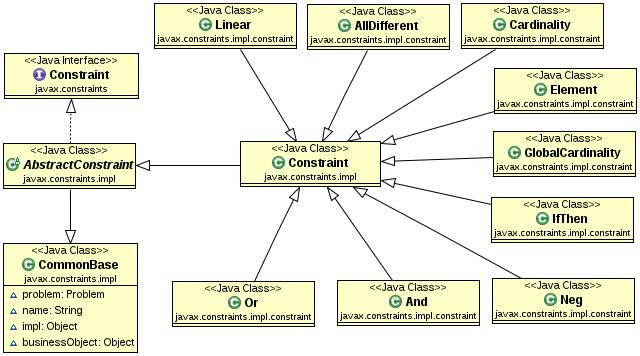
\includegraphics[scale=.5]{img/Constraints.JPG}
\caption{Class Diagram delle classi che implementano i vincoli.}
\end{figure}
